\chapter{Piattaforma di Simulazione}

\section{Architettura}

Al fine di poter simulare gli innumerevoli aspetti legati all'Electrical Mobility sono state usate diversi simulatori/tecnologie in simbiosi. In questa sezione verranno introdotte con una breve descrizione. Nelle sezioni successive verranno analizzate dettagliatamente mettendone alla luce gli aspetti utili al nostro fine.

\subsection{SUMO}\label{sumo}

SUMO (Simulator of Urban Mobility) è un simulatore Open Source e multi-piattaforma di traffico urbano progettato per simulare reti stradali di grandi dimensioni. Sviluppato in C++ è supportato principalmente dall'Institute of Transportation Systems at the German Aerospace Center. La simulazione è di tipo microscopico ovvero ogni veicolo è modellato in modo esplicito, ha un proprio itinerario e si muove individualmente attraverso la rete. Ogni aspetto relativo alla simulazione viene configurato attraverso file XML i quali descrivono la rete stradale, i parametri ed i percorsi di ogni singolo veicolo, ed eventualmente altri aspetti legati alla simulazione come i flussi di traffico oppure la descrizione degli edifici. 

SUMO permette di avviare la simulazione in due modalità:

\begin{itemize}
	\item \textbf{Visuale}: La modalità visuale permette di avere un riscontro visuale l'andamento della simulazione tramite un interfaccia che mostra la mappa della rete/città con vista dall'alto. Vengono mostrati tutti i veicoli ed è possibile accedere a tutti i parametri della simulazione. Vengono mostrati inoltre i semafori agli incroci, la segnaletica delle strade e, nel caso siano stati caricati, gli edifici della città. Tutto questo ovviamente impatta notevolmente sulle performance ma, al di la del gradevole effetto visivo, è utile per vedere come evolve la simulazione. Nel nostro caso, ad esempio, è servito per assicurarsi che i veicoli si fermassero alle colonnine, oppure per valutare la quantità di traffico generata in seguito all'inserimento di un determinato numero di veicoli. Molto utile è stato anche in fase di Demo per mostrare il funzionamento del nostro simulatore.
		
	\item \textbf{Testuale}: Con la modalità testuale vengono stampati nel terminale i messaggi di Warning ed Error nel terminale e se richiesto anche qualche messaggio di debug in più che indica gli step di avanzamento della simulazione. Dopo aver constatato che la simulazione si comporta come ci si aspetta tramite la modalità visuale si passa allora a questa modalità che ha performance assai maggiori. È quindi particolarmente indicata per le simulazioni di lunga durata.
\end{itemize}

\subsubsection{Tools}\label{sumo-tools}

I file XML che descrivono le simulazioni possono diventare molto complessi qualora si decida di simulare scenari realistici (come Bologna). SUMO mette a disposizione innumerevoli tool automatici per la generazione dei file di configurazione.  In questa tesi prenderemo in esame solo quelli che ci sono stati utili:

\begin{itemize}
 	\item \textbf{netconvert}: Genera file con estensione .net.xml della dove viene mappata la rete stradale. La generazione avviene in modo pseudo-casuale, tramite la definizione dei nodi e degli archi che definiscono il "grafo" della rete stradale oppure, come nel nostro caso, attraverso la conversione da formati esterni(OpenStreetMap, VISUM, VISSIM, OpenDRIVE, MATsim ecc..)
 	\item \textbf{polyconvert}: Genera file con estensione .poly.xml dove sono contenute le informazioni relative agli edifici, zone di verde, fiumi laghi ecc.. Anch'esse vengono importate dai file delle mappe in altri formati.
 	 \item \textbf{duarouter}: Genera file con estensione .rou.xml che descrivono per ogni veicolo il suo percorso, compresi tutti i suoi step intermedi. La generazione dei percorsi avviene applicando un algoritmo di cammino su grafi a scelta tra Dijikstra o A*. I punti di partenza e arrivo vengono generati casualmente da uno script in python messo a disposizione tra i tool di sumo (randomTrips.py).
\end{itemize}

\subsubsection{TRaCI}

TraCI (Traffic Controller Interface) è un modulo messo a disposizione da SUMO che permette di interagire con la simulazione in tempo reale tramite un protocollo Client/Server basato su TCP/IP. All'avvio della simulazione SUMO si mette in ascolto su una porta in attesa di messaggi, qualunque linguaggio che supporti il protocollo TCP/IP può dunque modificare lo stato della simulazione oppure ricevere notifiche sul cambiamento di variabili alle quali ci si può sottoscrivere. È proprio TraCI che farà da ponte tra SUMO e l'altro simulatore usato all'interno della nostra piattaforma.


\subsection{OMNeT++}
OMNeT++ è un ambiente OpenSource di simulazione a eventi discreti. È principalmente usato per la simulazione di reti di comunicazione, ma grazie alla sua architettura modulare ed estremamente flessibile è possibile utilizzarlo negli ambiti più disparati come la simulazione di sistemi informatici complessi, architetture hardware o, come nel nostro caso, per supporto alla simulazione veicolare.

Le simulazioni vengono modellate tramite l'impiego di componenti riusabili chiamati \emph{moduli} i quali possono essere combinati tra loro come dei blocchi LEGO.

I moduli possono essere connessi tra di loro attraverso i \emph{gates} e combinati insieme per formare dei moduli composti (compound modules). La comunicazione tra moduli normalmente avviene tramite message passing e i messaggi possono contenere strutture dati arbitrarie (a parte informazioni predefinite tipo i timestamp). Questi messaggi possono viaggiare attraverso percorsi predefiniti dai gates e dalle connections oppure essere inviati direttamente alla loro destinazione, quest'ultima scelta è molto utile nel caso delle comunicazioni wireless. 

I moduli, i relativi parametri e i collegamenti fra loro, vengono definiti tramite un linguaggio di alto livello (NED) in appositi file con estensione .ned, mentre la logica viene implementata in una corrispondente classe C++.

OMNeT++ viene distribuito con un IDE basato su Eclipse grazie al quale possono essere eseguite molte operazioni in modo visuale, come ad esempio la creazione e aggregazione di moduli.

Anche OMNeT++ mette a disposizione due modalità di esecuzione della simulazione una visuale (\emph{Tkenv}) e una testuale (\emph{Cmdenv}). La modalità visuale permette di vedere i moduli con i relativi messaggi che vengono scambiati, viene usata in fase di debug o in fase di Demo. La modalità testuale, ovviamente più performante e adatta alle simulazioni batch, mostra solo i messaggi di debug della simulazione insieme allo standard output dei moduli. Per i nostri scopi abbiamo usato solo la modalità testuale.

Un grande punto di forza di OMNeT++ sono gli strumenti messi a disposizione per l'analisi dei dati generati dalle simulazioni, che permettono di applicare, in tempo reale, trasformazioni e aggregazioni tra i set di dati e, in fine, visualizzare i risultati con varie tipologie di grafici: a barre, a linee, istogrammi e molti altri.

\subsection{Veins}\label{veins}
Veins è un framework OpenSource per la simulazione di reti veicolari IVC (Inter-Vehicular Communication). Utilizza OMNeT++ e SUMO in simbiosi. Si appoggia su MiXiM, un framework per OMNeT++, che implementa modelli per reti wireless fisse e mobili (reti di sensori wireless, reti ad hoc, reercorso, colore, velocità, accelerazione, parcheggio ecc..ti veicolari ecc.). La comunicazione con SUMO avviene tramite TRaCI. Ogni volta che nella simulazione in SUMO viene aggiunto un veicolo Veins crea dinamicamente un corrispondente modulo OMNeT++ che permette di controllarlo sotto ogni aspetto (ercorso, colore, velocità, accelerazione, parcheggio ecc..).

Il nostro simulatore consiste in un modulo di Veins, il quale è stato opportunamente modificato al fine di avere un ambiente che contiene solo i componenti strettamente necessari allo scopo in quanto le performance sono determinanti al fine di poter avere dei risultati in tempi utili. Infatti sono stati rimossi da Veins i moduli necessari alla comunicazione wireless (nic80211 e ARP), il modulo per la gestione degli ostacoli (obstacles) che era utilizzato per la gestione dello shadowing delle reti wireless


\section{L'ambiente di simulazione}

In questa sezione verranno descritti in dettaglio i componenti del simulatore, da noi creati, ovvero i moduli di OMNeT++, gli script per generare i file di configurazione di SUMO e gli script per lanciare le simulazioni batch.

La logica del simulatore è implementata attraverso moduli di OMNeT++. Grazie ad essi sono implementati, i modelli di consumo dei veicoli elettrici, i comportamenti degli degli autisti e la rete di distribuzione elettrica cittadina. L'unico aspetto non implementato è la guida dei veicoli in quanto è gestita da SUMO.

I file di configurazione di SUMO sono generati da script che in base ai parametri specificati possono variare l'intensità del traffico.



\subsection{Generazione file di Configurazione}

Dopo aver scaricato compilato ed installato tutti i componenti è necessario generare i file di configurazione riguardanti lo scenario che si vuole simulare. 

\subsection{Download Scenario}

A questo punto è necessario scegliere quale scenario si vuole simulare. Lo scenario di Bologna è già disponibile nella cartella \code{simulator/veins-2.1/examples/veins/bologna} siccome è quello di nostro interesse.

Nel caso in cui si sia interessati ad uno scenario diverso da quello di Bologna il modo più semplice per ottenere la mappa desiderata è andare all'indirizzo \url{http://www.openstreetmap.org/export} e scaricarsi l'area interessata. La dimensione delle mappe scaricabili è limitata onde evitare la saturazione della banda del server. Per sopperire a questa mancanza SUMO mette a disposizione un tool situato in \code{<SUMO_HOME>/tools/import/osm/osmGet.py} che permette di scaricare mappe di dimensione arbitraria. Per l'utilizzo di questo tool rimando alla documentazione dello script oppure alla pagine ufficiale:

\url{http://sumo-sim.org/userdoc/Networks/Import/OpenStreetMapDownload.html}.

\subsubsection{Profilo Altimetrico}\label{profilo-altimetrico}

Da notare che le mappe di Open Street Map non contengono le informazioni relative al profilo altimetrico. È quindi necessario "arricchire" la mappa scaricata con tali informazioni. Il programma utilizzato a questo scopo è Osmosis, presente nella cartella \code{osmosis} del progetto. In particolare ho usato \code{osmosis-srtm-plugin_1.1.0} che permette, attraverso l'interrogazione di file SRTM (scaricabili da \url{http://dds.cr.usgs.gov/srtm/version2_1/SRTM3/}, di inserire i dati del profilo altimetrico nelle mappe di Open Street Map. 

Di seguito viene mostrato l'utilizzo del Osmosis e del relativo plugin considerando \code{\$SRTM_HOME} la cartelle che contiene i file SRTM e \code{\$CITY_NAME} il nome della città. Quindi avendo, ad esempio, \code{bologna.osm}, ovvero la mappa della città di Bologna senza dati riguardanti il profilo altimetrico, in output avremo \code{bologna_srtm.osm}, ovvero la stessa mappa con i dati estratti dai file SRTM.

\begin{bash}
osmosis -plugin org.srtmplugin.osm.osmosis.SrtmPlugin_loader --read-xml "\$CITY_NAME".osm --write-srtm locDir="\$SRTM_HOME" locOnly=true repExisting=false --write-xml "\$CITY_NAME"_srtm.osm
\end{bash}

%

Da tenere in considerazione il fatto che il comando mostrato è incluso nello script di generazione automatica da me creato al fine di velocizzare la configurazione dello scenario.

\subsection{Generazione XML di SUMO}

SUMO necessita di file di configurazione in XML che descrivono la rete stradale, i poligoni dei palazzi e i percorsi di ogni singolo veicolo. Siccome ognuno di questi file, per essere generato, richiede un apposito comando il quale a sua volta richiede vari parametri, ho creato uno script che data la mappa di una città in formato Open Street Map esegue tutte le operazioni necessarie.

Verranno comunque analizzati tutti i comandi singolarmente in modo d aavere una panoramica sulle scelte implementative.

\subsubsection{La rete Stradale (.net.xml)}

Il file della rete stradale viene generato attraverso il tool \code{netconvert} direttamente dalla mappa di Open Stree Map. Oltre al file \code{.osm} è necessario anche un file di supporto che istruisca SUMO sui vincoli e i limiti di velocità delle strade importate. Noi ne utilizziamo uno creato ad hoc per il traffico tedesco. 

Qui sotto ne riporto un frammento a puro titolo esemplificativo, il file intero si trova in \code{simulator/veins-2.1/examples/veins/bologna/osm-urban-de.typ.xml}

\begin{xml}
<types xmlns:xsi="http://www.w3.org/2001/XMLSchema-instance">
  <type id="highway.motorway" priority="13" numLanes="2" speed="41.667"
                oneway="true" disallow="bicycle pedestrian"/>
  <type id="highway.motorway_link" priority="8" numLanes="1" speed="13.889"/>
  <type id="highway.trunk" priority="12" numLanes="2" speed="13.889"/>
  <type id="highway.trunk_link" priority="8" numLanes="1" speed="13.889"/>
  <type id="highway.primary" priority="11" numLanes="2" speed="13.889"/>
  <type id="highway.primary_link" priority="8" numLanes="1" speed="13.889"/>
  <type id="highway.secondary" priority="10" numLanes="2" speed="13.889"/>
  ....
</types> 
\end{xml}

Di seguito passiamo ad un analisi dettagliata di tutti i parametri passati a \code{netconvert}:

\begin{itemize}
	\item \textbf{-{}-type-files}: Specifica il file che contiene i vincoli e i limiti, quello citato sopra.
	\item \textbf{-{}-ramps.guess}: Prova a capire dove sono le rampe e ad eseguirne l'importazione
	\item \textbf{-{}-remove-edges.by-vclass}: Siccome Open Street Map include un infinità informazioni del tutto inutili al nostro fine (ferrovie, piste ciclabili, aree pedonali ecc..) con questo parametro si indicano le classi da non importare (\code{bicycle,pedestrian...})
	\item \textbf{-{}-geometry.remove}:
	\item \textbf{-{}-remove-edges.isolated}:
	\item \textbf{-{}-tls.join}:
	\item \textbf{-{}-osm-files}:
	\item \textbf{-{}-output.street-names}:
	\item \textbf{-{}-output.original-names}:
	\item \textbf{-{}-output-file}:
\end{itemize}

Siccome Open Street Map include molte informazioni che sono del tutto inutili al nostro fine (ferrovie, piste ciclabili, aree pedonali ecc..) bisogna istruire \code{netconvert} affinché le escluda dall'importazione. 

%\begin{bash}
%netconvert --type-files osm-urban-de.typ.xml --ramps.guess --remove-edges.by-vclass hov,taxi,bus,delivery,transport,lightrail,cityrail,rail_slow, rail_fast,motorcycle,bicycle,pedestrian --geometry.remove --remove-edges.isolated true --tls.join --osm-files "$MAP_FILE" --output.street-names --output.original-names --output-file "$CITY_NAME".net.xml
%\end{bash}


 
\subsection{Il funzionamento di Veins}

Veins è il ponte tra OMNeT++ e SUMO e la comunicazione tra i due avviene tramite TraCI. In realtà "in mezzo" ai due simulatori si trova uno script python, \emph{sumo-launchd.py}, che sta in ascolto sulla prima porta libera che trova, in attesa che venga avviato Veins. Quando Veins viene avviato si connette a questo script il quale lancia SUMO, a questo punto inizia la sincronizzazione tra i due simulatori che avviene tramite "staffetta" come mostrato in Fig. ~\ref{fig:veins-state-machine}. Per garantire l'esecuzione sincrona a intervalli definiti Veins inserisce in un buffer tutti i comandi da inviare a SUMO (Fig.  ~\ref{fig:veins-sequence-diagram}). Ad ogni passo temporale, i comandi contenuti nel buffer vengono inviati. Ciò innesca l'avanzamento del corrispondente passo temporale nella simulazione del traffico stradale. Al termine dello step temporale di simulazione del traffico stradale, SUMO invia una serie di comandi con lo stato e la posizione di tutti i veicoli istanziati in risposta a Veins. Dopo l'elaborazione di tutti i comandi ricevuti Veins aggiunge i corrispettivi nodi per ogni nuovo veicolo introdotto nella simulazione e rimuove invece i nodi relativi ai veicoli che sono giunti a destinazione. A questo punto la simulazione può avanzare al prossimo step temporale.

\begin{figure}[H]
        \centering
        \begin{subfigure}[H]{0.5\textwidth}
                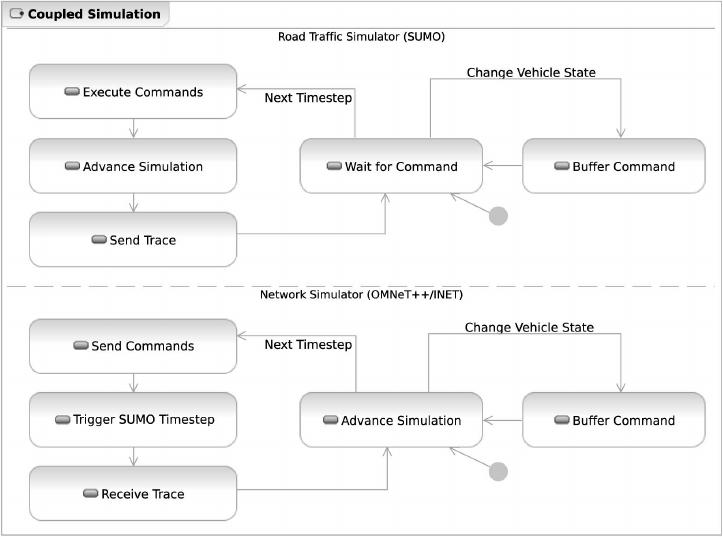
\includegraphics[width=\textwidth]{assets/veins-state-machine.jpg}
                \caption{Panoramica dei due simulatori abbianti. Macchina a stati di SUMO e i moduli di Veins.}
                \label{fig:veins-state-machine}
        \end{subfigure}%
        ~ %add desired spacing between images, e. g. ~, \quad, \qquad etc.
          %(or a blank line to force the subfigure onto a new line)
        \begin{subfigure}[H]{0.5\textwidth}
                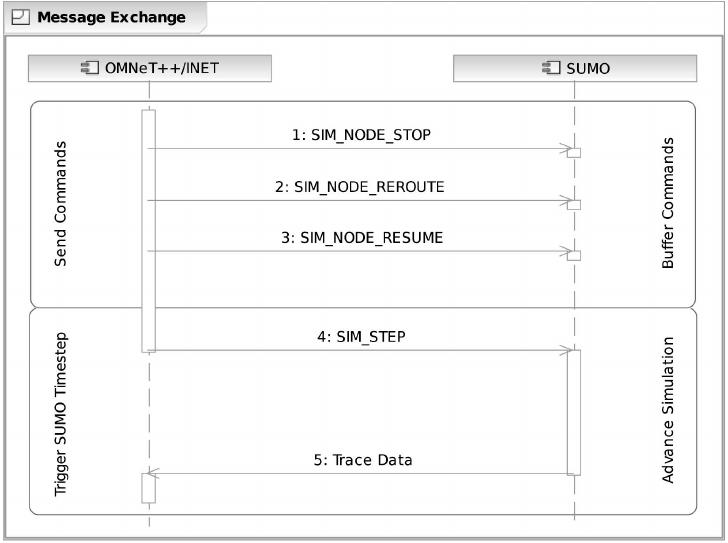
\includegraphics[width=\textwidth]{assets/veins-sequence-diagram.jpg}
                \caption{ Diagramma di sequenza dei messaggi scambiati tra SUMO e Veins. L'esecuzione dei comandi è ritardata fino al successivo passo temporale in SUMO.}
                \label{fig:veins-sequence-diagram}
        \end{subfigure}
        \caption{Architettura Veins}
\end{figure}


%Questo compito è svolto dalla classe \emph{TraCIScenarioManager} che all'avvio del simulatore instaura la connessione %con SUMO tramite TraCI. 

\section{I Moduli}

\subsubsection{Car}

(Fig: ~\ref{fig:module-car}).

\begin{figure}[H]
\centering
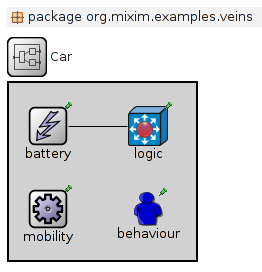
\includegraphics[scale=0.5]{assets/module-car.png}
\caption{Modulo Car}
\label{fig:module-car}
\end{figure}


\subsection{CarLogic}

CarLogic è il modulo che implementa la logica di ogni veicolo gestito dal simulatore attraverso un automa a stati finiti. 


\begin{description}
  \item[userName]  \hfill \\ 
      Nome completo dell'utente che possiede il veicolo
  \item[userId]  \hfill \\
      Username dl''utente che possiede il veicolo
  \item[manufacturer]  \hfill \\
      Fabbricante
  \item[model]  \hfill \\ 
      Modello
  \item[cRoll]  \hfill \\
      Attrito di qualcosa
  \item[cDrag]  \hfill \\
      Attrito di qualcos altro
  \item[across]  \hfill \\
      Attrito di qualcos altro ancora
  \item[rhoAir]  \hfill \\
      Attrito dell'aria
  \item[weight]  \hfill \\
      Peso del veicolo
  \item[threshold]  \hfill \\
      Soglia sotto la quale il veicolo richiede la ricarica \ldots
\end{description}

\subsection{Battery}

\subsection{CityService}

